\chapter{Industrierobotik}
\section{Industrieroboter}
\begin{itemize}
	\item \textbf{Roboterarm} mit Achsen, Gelenken und Antrieben
	\item Steuerung in einem \textbf{Steuerschrank} mit \textbf{Bedienerkonsole}
	\item \textbf{Handsteuergerät}
\end{itemize}
\subsection{Einsatz}
\begin{itemize}
	\item In wohldefinerter Umgebung, definierte Hindernisse, bekannte Umwelt
	\item Größtes Einsatzgebiet in der Automobilindustrie und deren Zulieferern (\textit{Schweißen, Lackieren, Beschichten ...})
\end{itemize}
\subsection{Trends}
\begin{itemize}
	\item Industrie 4.0, KI, IoT
	\item Human-Robot collaboration
	\item Mobile Roboter und einfachere Bedienung
\end{itemize}
\section{Bauform und Komponenten}
\paragraph{Roboterarm}
\begin{itemize}
	\item Armelemente bzw. Glieder die über Bewegungsachsen miteinander verbunden sind.
	\item Ausgleichszylinder $\Rightarrow$ Motoren werden nicht überlastet, geringere Kräfte sind nötig
\end{itemize}
\paragraph{Endeffektor, Hand}
\begin{itemize}
	\item Das Arbeitsorgan $\Rightarrow$ Werkzeug
	\item Üblicherweise wird die Werkzeugspitze \textit{\textbf{Tool Center Point}(TCP)} genannt
\end{itemize}
\paragraph{Fahrzeug}
\begin{itemize}
	\item optional
	\item meist bodengebunden
	\item ein bis drei Freiheitsgrade
	\item Bsp.: Verfahrschlitten
\end{itemize}
\section{Freiheitsgrade}
\subsection{Definition}
Der Freiheitsgrad (DOF) bezeichnet in der Physik die Anzahl der frei wählbaren, voneinander unabhängigen Parameter eines physikalischen Systems, die dessen Zustand eindeutig kennzeichnen.
\begin{itemize}
	\item In der Mechanik drückt der DOF die Möglichkeit aus im Raum voneinander unabhängig Bewegungen auszuführen
	\item Anzahl der Freiheitsgrade drückt die translatorischen und rotatorischen Bewegungsmöglichkeiten eines Körpers aus
	\item Anzahl der Gelenkachsen $\neq$ Anzahl der Freiheitsgrade
\end{itemize}
\section{Bewegungsachsen}
\subsection{Rotatorisch}
\begin{figure}[H]
	\begin{center}
		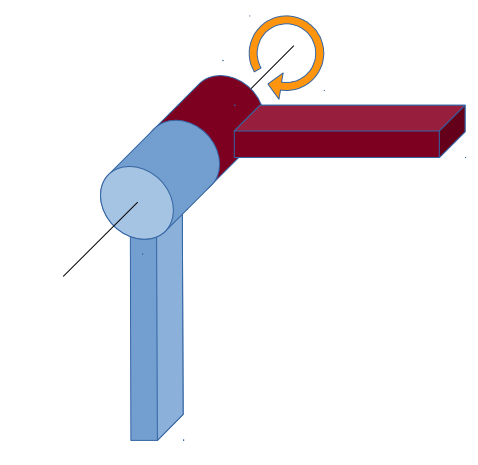
\includegraphics[scale=0.6]{Resources/PNG/Rotatorisch.PNG}
		\caption{Rotatorische Achse}
		\label{fig:PNG/Rotatorisch.PNG}
	\end{center}
\end{figure}
\begin{itemize}
	\item Für Drehbewegungen
	\item Freiheitsgrad: 1
\end{itemize}
\subsection{Translatorisch}
\begin{figure}[H]
	\begin{center}
		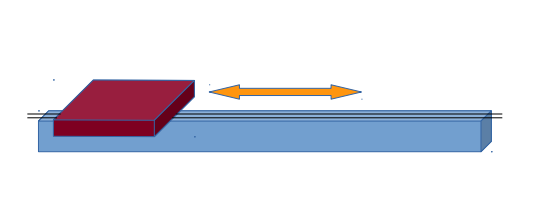
\includegraphics[scale=0.6]{Resources/PNG/Translatorisch.PNG}
		\caption{Translatorische Achse}
		\label{fig:PNG/Translatorisch.PNG}
	\end{center}
\end{figure}
\begin{itemize}
	\item Für Schubbewegungen
	\item Freiheitsgrad: 1
\end{itemize}
\paragraph{Hauptachsen}
\begin{itemize}
	\item Zum Positionieren des Effektors im Raum
	\item Beeinflussen Position des TCP
	\item Rotatorisch oder Translatorisch
\end{itemize}
\paragraph{Nebenachsen}
\begin{itemize}
	\item Kopf- oder Handachsen
	\item Rufen nur kleine Positionsänderungen hervor
	\item Orientierung des Werkzeugs
	\item Meist rotatorisch
\end{itemize}
\subsection{Rotationsgelenk}
Die Drehachse bildet einen rechten Winkel mit den Achsen der beiden angeschlossenen Glieder.
\begin{figure}[H]
	\begin{center}
		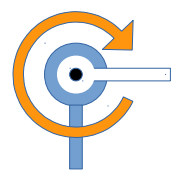
\includegraphics[scale=0.6]{Resources/PNG/Rotationsgelenk.PNG}
		\caption{Rotationsgelenk}
		\label{fig:Resources/PNG/Rotationsgelenk}
	\end{center}
\end{figure}
\subsection{Torsionsgelenk}
Die Drehachse verläuft parallel zu den Achsen der beiden Glieder.
\begin{figure}[H]
	\begin{center}
		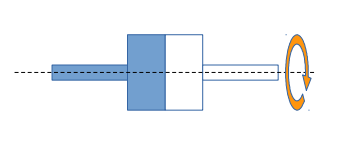
\includegraphics[scale=0.6]{Resources/PNG/Torsionsgelenk.PNG}
		\caption{Torsionsgelenk}
		\label{fig:Resources/PNG/Torsionsgelenk}
	\end{center}
\end{figure}
\subsection{Revolvergelenk}
Das Eingangsglied verläuft parallel zur Drehachse, das Ausgangsglied steht im rechten Winkel zur Drehachse.
\begin{figure}[H]
	\begin{center}
		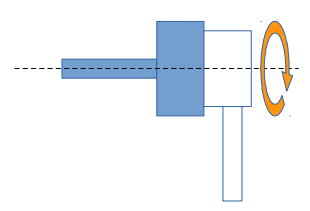
\includegraphics[scale=0.6]{Resources/PNG/Revolvergelenk}
		\caption{Revolvergelenk}
		\label{fig:Resources/PNG/Revolvergelenk}
	\end{center}
\end{figure}
\subsection{Kugelgelenk}
Besitzt 3 Freiheitsgrade, wobei die Beweglichkeit stark eingeschränkt ist.
Arbeitsbereich der X- und Y-Achse wird durch die Konstruktion auf unter 
180 $\deg$ limitiert.
Die Einkerbung an der Vorderseite lässt an dieser stelle einen 90 $\deg$ Winkel zu.
\begin{figure}[H]
	\begin{center}
		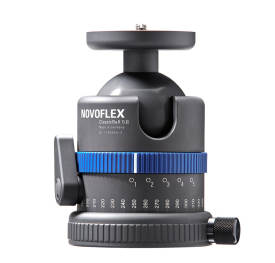
\includegraphics[scale=0.8]{Resources/PNG/Kugelgelenk.PNG}
		\caption{Kugelgelenk}
		\label{fig:Resources/PNG/Kugelgelenk.PNG}
	\end{center}
\end{figure}
\section{Arbeitsraum}
\paragraph{Definition} Punkte im 3D-Raum, die von der Roboterhand angefahren werden können.
\section{Grundtypen von Industrierobotern}
\subsection{Portalroboter}
\begin{itemize}
	\item Steife Struktur $\Rightarrow$ sehr große Arbeitsräume möglich
	\item Sehr hohe Genauigkeit
	\item Einfache Steuerung in kartesischen Koordinaten
\end{itemize}
\subsection{Horizontal-Knickarmroboter}
\begin{itemize}
	\item \textbf{SCARA}: Selective Compliance Assembly Robot Arm
	\item Aufbau: Ähnlich des menschlichen Arms, horizontaler Gelenkarmroboter
	\item In der Regel 4 Achsen und Freiheitsgrade $f = 4$
	\item Hohe Steifigkeit in vertikaler Richtung
	\item Hohe Geschwindigkeiten möglich
\end{itemize}
\subsection{Vertikal-Knickarmroboter}
\begin{itemize}
	\item Klassischer, universell einsetzbarer Industrieroboter
	\item 4-6 rotatorische Achsen und Freiheitsgrade
	\item Drei Hauptachsen und drei Nebenachsen
\end{itemize}
\subsection{Parallele Roboter}
\begin{itemize}
	\item Bekannt von Flugsimulatoren, Nachbildung der Beschleunigung durch Kippen einer Plattform gegen den Erdbeschleunigungsvektor
	\item Geschlossene Führungsketten mit fest montierten Antrieben
	\item Paralleler Roboter, da die Antriebsachsen parallel auf den Endeffektor wirken
\end{itemize}
\paragraph{Hexapod}
\begin{itemize}
	\item Hohe Stabilität aber geringe Geschwindigkeit
	\item Aus 6 Linearachsen aufgebaut
\end{itemize}
\paragraph{Delta-Roboter}
\begin{itemize}
	\item Schnelle Handhabung
	\item Drei bis vier Gelenkachsen mit stationären Antrieben
	\item Evtl. Erweiterung mit einer 3-Achs Hand
\end{itemize}
\subsection{Leichtbauroboter}
\begin{itemize}
	\item Typ. Massenverhältnis Industrieroboter Last/Eigenmasse: 1:10
	\item DLR Leichtbauroboter III: Last/Eigenmasse = 1:1
\end{itemize}
\section{Effektoren}
\subsection{Endeffektoren}
\begin{itemize}
	\item Arbeitsorgan am Ende eines Roboterarms, mit dem direkt auf ein Werkstück eingewirkt werden kann.
	\item Angebracht an der entferntesten Stelle einer kinematischen Kette
	\item \textbf{Typen}:
	\subitem Werkzeuge
	\subitem Greifer
	\subitem Prüfmittel
	\item  Zustände der Effektoren werden mit Sensoren erfasst.
\end{itemize}
\subsection{Greifersysteme}
Ein Griff muss \textbf{stabil} sein und \textbf{kollisionsfrei} ausgeführt werden können.
Objekt darf nicht im Greifer abgleiten oder sich verschieben.
%Einschränkungen, wo das Objekt nicht gegriffen werden darf, müssen beachtet werden.
\paragraph{Typen}
\begin{itemize}
	\item \textbf{Mechanisch}
	\item \textbf{Vakuum}
	\item \textbf{Magnetisch}
\end{itemize}
\subsection{Greifplanung}
Ein technischer Griff unterteilt sich in die Sequenzen:
\begin{itemize}
	\item Herstellen des Kontakts zwischen Greifobjekt und Greifer
	\item Sichern des Haltens während der Bewegung in allen Richtungen
	\item Genaues Ablegen des Objekts in der Zielposition und in kürzester Zeit
\end{itemize}
\subsection{Greifprinzipien}
\paragraph{Formschlüssiger Griff}
\begin{itemize}
	\item Das Objekt liegt lose zwischen den Greifbacken
	\item Geringe Kräfte auf das Objekt
	\item Positionserhaltung durch passende Geometrie der Greiferbacken
\end{itemize}
\paragraph{Stoffschlüssiger Griff}
\begin{itemize}
	\item Zwischen Greifer und Objekt wirken Kräfte in Form von Klebstoffen oder Flüssigkeitsbrücken
\end{itemize}
\paragraph{Kraftschlüssiger Griff}
\begin{itemize}
	\item Kontakt zwischen Greifer und Objekt durch Punkt- oder Flächenkräfte
	\item Reibkräfte, Vakuum oder Magnetkräfte
	\item Aneinander pressen, so dass die Reibungskräfte ein Verschieben der Bauteile gegeneinander verhindern
\end{itemize}
\section{Antrieb}
\subsection{Antriebsarten}
\begin{itemize}
	\item Antrieb muss Kräfte und Momente durch das Gewicht der Roboterarme und der Objekte im Effektor kompensieren
	\item Antrieb besteht aus Motor, Getriebe und Wegmesssystem
	\item Drei Antriebsarten:
	\subitem pneumatisch
	\subitem hydraulisch
	\subitem elektrisch
\end{itemize}
\subsection{Sensor}
Umwandeln einer mechanischen, physikalischen oder chemischen Größe in ein Signal.
Gegenteil eines Aktors.
\paragraph{Interne Sensoren} Erfassen interner Zustände des Roboters
\begin{itemize}
	\item Weg- und Winkelmessung
	\item Geschwindigkeit
	\item Batteriespannung
\end{itemize}





















